\section{Experiments}
\label{sec:exp}

The efficiency and scalability of Legion was examined by measuring the performance
of three applications on three clusters.  The table in Figure~\ref{fig:systems} summarizes 
the three clusters that were used.

\begin{figure}
{\footnotesize
\begin{tabular}{l|ccc}
Cluster & Sapling & Viz & Keeneland \\
\midrule
Nodes   &   4     &  10 &  32 (120) \\
CPUs/Node & 2x Xeon 5680 & 2x Xeon 5680 & 2x Xeon 5660 \\
HyperThreading & on & off & off \\
GPUs/Node & 2x Tesla C2070 & 5x Quadro Q5000 & 3x Tesla M2090 \\
DRAM/Node & 48 GB & 24 GB & 24 GB \\
Infiniband & 2x QDR & QDR & QDR \\
\end{tabular}
}

\caption{Configurations of Systems Used for Experiments \label{fig:systems}}
\end{figure}

Nodes with multiple instances of different resources are a challenge for 
existing programming models that have a flat model of the system (e.g. MPI).
They are faced with a choice of lumping all 
the resources together and ignoring the internal irregularities (e.g. NUMA
in multi-socket x86 systems) or of separating a single physical node into
multiple smaller nodes, ignoring the better affinity between sockets/GPUs/etc
on the same node and either wasting or over-subscribing some resources when
the quantities of different resources don't share a common divisor.

In contrast, the machine model used by the Legion runtime is based on an
affinity graph of CPUs and GPUs and is able to accurately capture complex
machine hierarchies.

For each application, multiple problem sizes were used, and each size problem was
run on subsets of each machine ranging from the smallest (a single CPU core or GPU)
to the largest or near-largest (except Keeneland which has 115 nodes, but we limited 
our runs to at most 32 nodes to get sufficient cluster time.)
By looking at the performance of the same size problem over progressively larger
machines, we are able to measure the strong scaling that Legion is able to
archive.  By increasing the problem size as well, we also measure weak scaling.

\subsection{Circuit Simulation}
\label{subsec:exp_ckt}

The first experiment we investigate is the distributed circuit simulation described in 
Section~\ref{sec:ex}.  The Legion runtime handles all of the resource allocation, 
scheduling, and data movement across the cluster of GPUs.  In particular,  
Legion's ability to efficiently move the irregularly partitioned
shared data around the system while keeping the private nodes and wires resident in
each GPU's framebuffer memory is critical in keeping the overhead low and achieving 
good scalability.

Circuits of two different sizes were simulated.  The first had 480K wires, connecting
120K nodes.  The second is twice as large, with nearly a million wires connecting a
quarter of a million nodes.  In addition to running these tests on varying number of
nodes, the number of GPUs used by the runtime was also varied.  In no case did the 
changes to nodes or number of GPUs per node require any changes to the application code.

The circuit simulation used a simple, but application-specific, mapper.  At initialization
time, the mapper queries the list of GPUs in the machine and identifies each GPU's
framebuffer memory and {\em zero-copy} memory, the pinned memory that both the GPU and
CPUs in the system can access directly.  Once the circuit is partitioned, the partitions
are assigned a home GPU in round-robin fashion.  Every task related to that partition is
then sent to the home GPU, with no task stealing allowed.  (If the circuit is partitioned well,
there is minimal load imbalance between the pieces, and the rebalancing benefit of 
moving a partition is unlikely to be worth the cost of moving all the 
private data for a piece from one GPU to another.)  The regions for a task are mapped as 
shown in Figure~\ref{fig:gpumapping}.

Figure~\ref{fig:ckt_speed} shows the performance of the Legion circuit simulation relative
to a hand-coded single-GPU implementation written in CUDA.  Each line shows the scaling of
a particular problem size as the number of nodes is varied.  Our results demonstrate
excellent strong scaling, with speedups of 39.0X for the small problem on 48 GPUs and 
62.5X for the larger problem size on 96 GPUs.  On a single GPU, our Legion implementation
was within 5\% of the performance of the hand-coded example.

Figure~\ref{fig:ckt_overhead} shows the fraction of the overall simulation time (summed over
all nodes) spent in the application kernels compared to the various pieces of the Legion
runtime.  As the node count increases, the non-communication overhead stays relatively constant.
As expected the communication overhead grow linearly with number of nodes.

\begin{figure}
\subfigure[Circuit Simulation Speed Relative to Single-GPU Implementation]
{
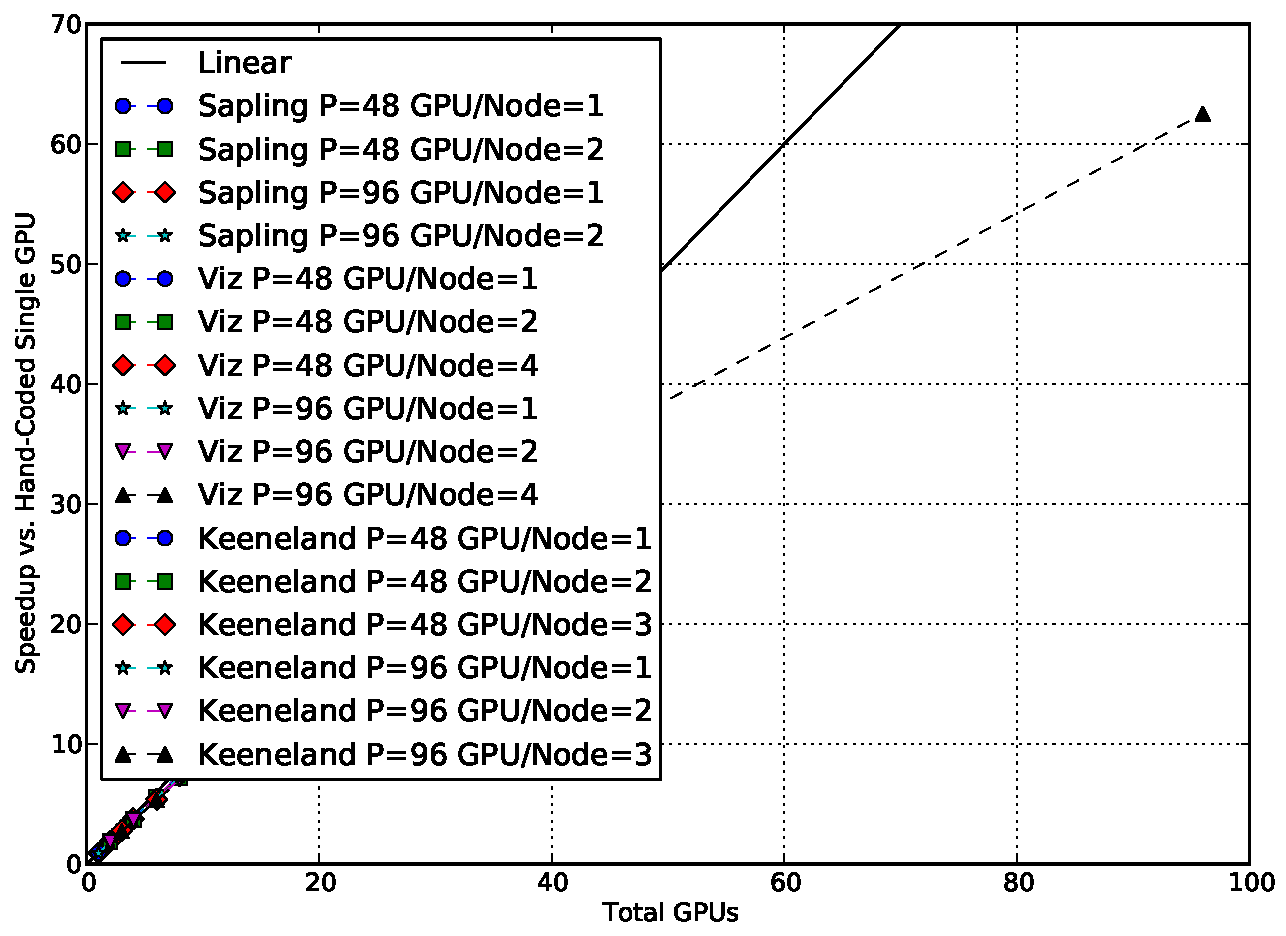
\includegraphics[scale=0.4]{figs/circuit_speedups.pdf}
\makebox[0pt][r]{
\raisebox{0.25 in}{
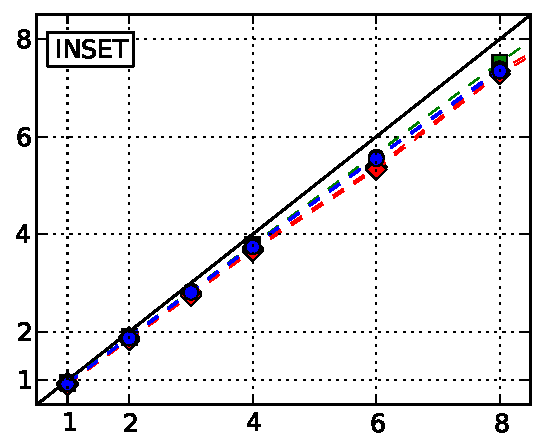
\includegraphics[scale=0.18]{figs/circuit_speedups_zoom.pdf}
}
}
\label{fig:ckt_speed}
}

\subfigure[Overhead of Circuit Simulation on Keeneland with 3 GPUs/Node]
{
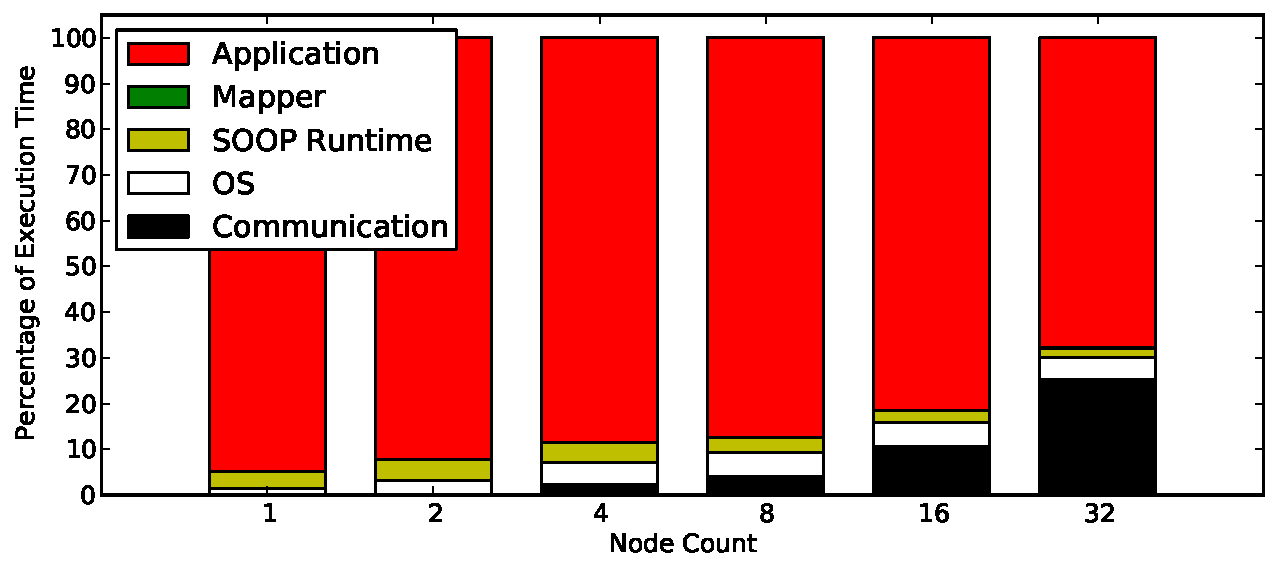
\includegraphics[scale=0.4]{figs/circuit_overhead.pdf}
\label{fig:ckt_overhead}
}
\caption{Circuit Simulation Results}
\end{figure}

\subsection{Particle Simulation}
\label{subsec:exp_fluid}

Our second experiment is a port of the \emph{fluidanimate} benchmark from the PARSEC suite\cite{bienia11benchmarking},
which does a particle-based simulation of an incompressible fluid.  Each particle interacts only with other nearby
particles. The benchmark divides the space in which the fluid can move into a three-dimensional array of cells 
such that the range of interaction is limited to just the
cells adjacent (including diagonals) to the one a particle resides in.  Originally designed to be a
chip multiprocessor benchmark, the application divides the array into {\em grids} and assigns each one to 
a thread.  Per cell locking is used to safely access particles in cells that lie
on the edge of a grid.  This fine-grained locking scheme along with the assumption of a shared address space lead to
good scaling in a multi-core processor, but rule out any attempt run beyond a single node.  To extend the
scaling further, our port uses region partitioning to divide the array into grids in a similar
way, but handles the interaction between grids in a way that doesn't rely on access to uniform shared memory.
Instead, the Legion version of the benchmark creates explicit ghost copies of cells on the boundaries of grids
and uses those ghost cells to exchange information between the grids.

The mapper for the particle simulation is very simple - it maps one grid's tasks onto each processor and
maps all regions for that grid (both the internal and the ghost regions) into the system memory used by that processor.
The exchange of the ghost cell data between processors is handled by the Legion runtime as a ghost cell region
gets alternately mapped in two different memories.

Figure~\ref{fig:fluid_single} compares the performance of the Legion implementation against the PARSEC version,
using a relatively small problem (300K particles on a 15x21x15 array of cells).  Between 1 and 4 threads, the
results for sapling are nearly indistinguishable, indicating 
neither the Legion runtime nor the the restructuring of the implementation to allow multi-node scaling impose
any significant overhead.  It's possible that the use of explicit ghost cells rather than 
fine-grained sharing of cache lines might be a net win.  At 8 threads and above, the performance begins to vary.
Both the Legion and PARSEC version on viz flatten out as they over-subscribe the 12 physical cores.  On sapling,
which has HyperThreading enabled, deviations from linear begin sooner as the operating system's scheduler's
thread placement choices begin to matter.

To measure scaling beyond a single node, three different problem sizes were run for each of the three systems,
 with the results plotted in Figure~\ref{fig:fluid_multi}.  
 For the smallest problem (300K particles), we observe a 20\% speedup when going to 1
node to 2 (a total of 16 threads), but begin slowing down beyond that due to communication overhead - at 4 nodes
there are twice as many ghost cells as interior grid cells.  The larger problem sizes (2.4M and 19M
particles) do much better, with scaling of up to 5.4x when going from 1 node up to 16 because the
communication-to-computation ratio is lower.

%Although the particle simulation being performed is on a regular array of cells, it turns out that the
%distribution of particles amongst the cells is very irregular.  The simulation models gravity, which points in
%the -Y direction, so the particles are clustered mostly in the lower half of the cell array.  The PARSEC
%implementation works around this imbalance by only slicing the cell array through the X and Z axes, yielding
%grids that are uniformly populated, even if the number of boundary cells (for which locks must be used) is
%increased above the minimum. MORE TEXT NEEDED HERE

\begin{figure}
\subfigure[Single-Node Particle Simulation Speed]
{
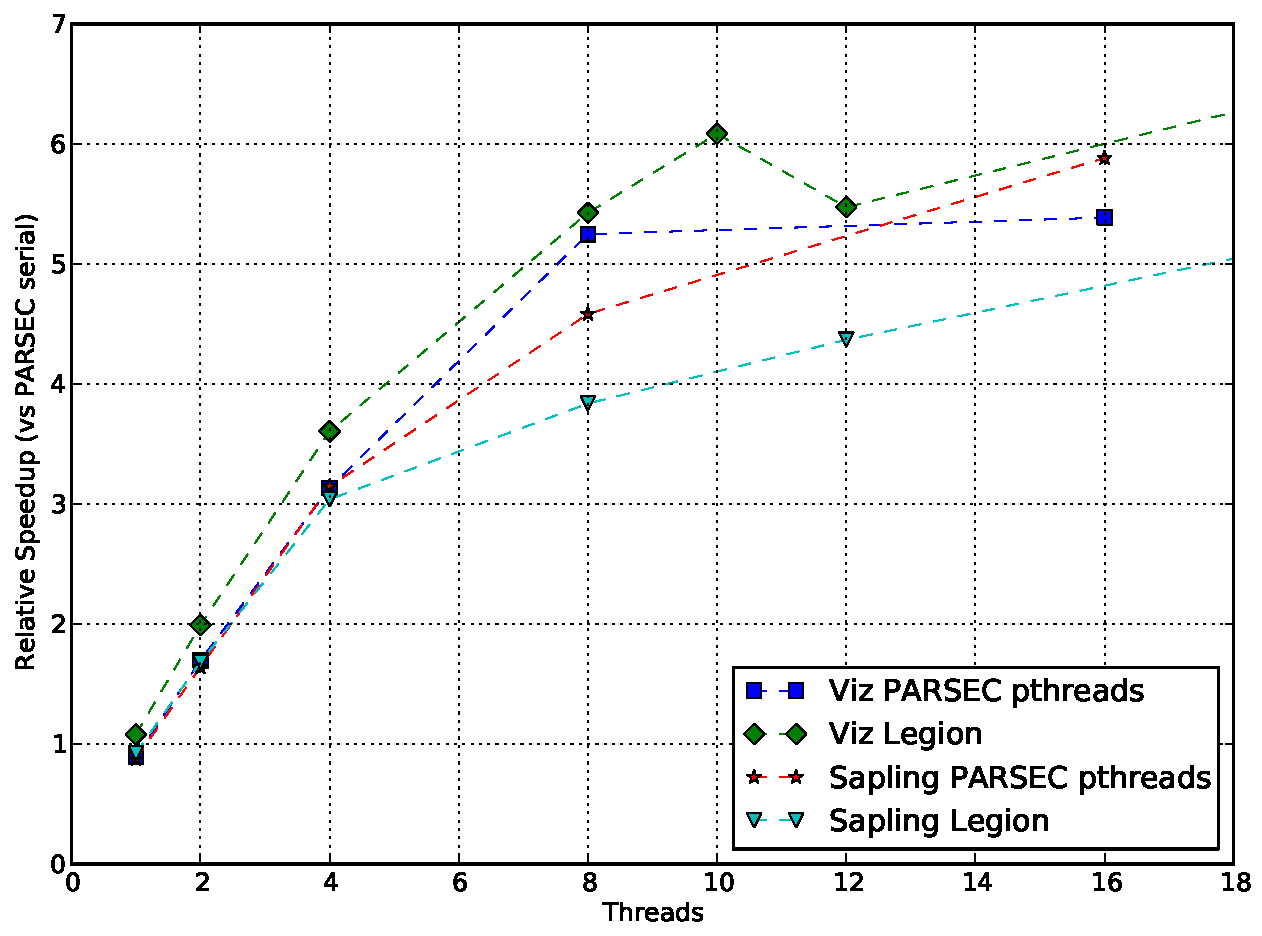
\includegraphics[scale=0.4]{figs/fluid_singlenode.pdf}
\label{fig:fluid_single}
}

\subfigure[Multi-Node Scaling]
{
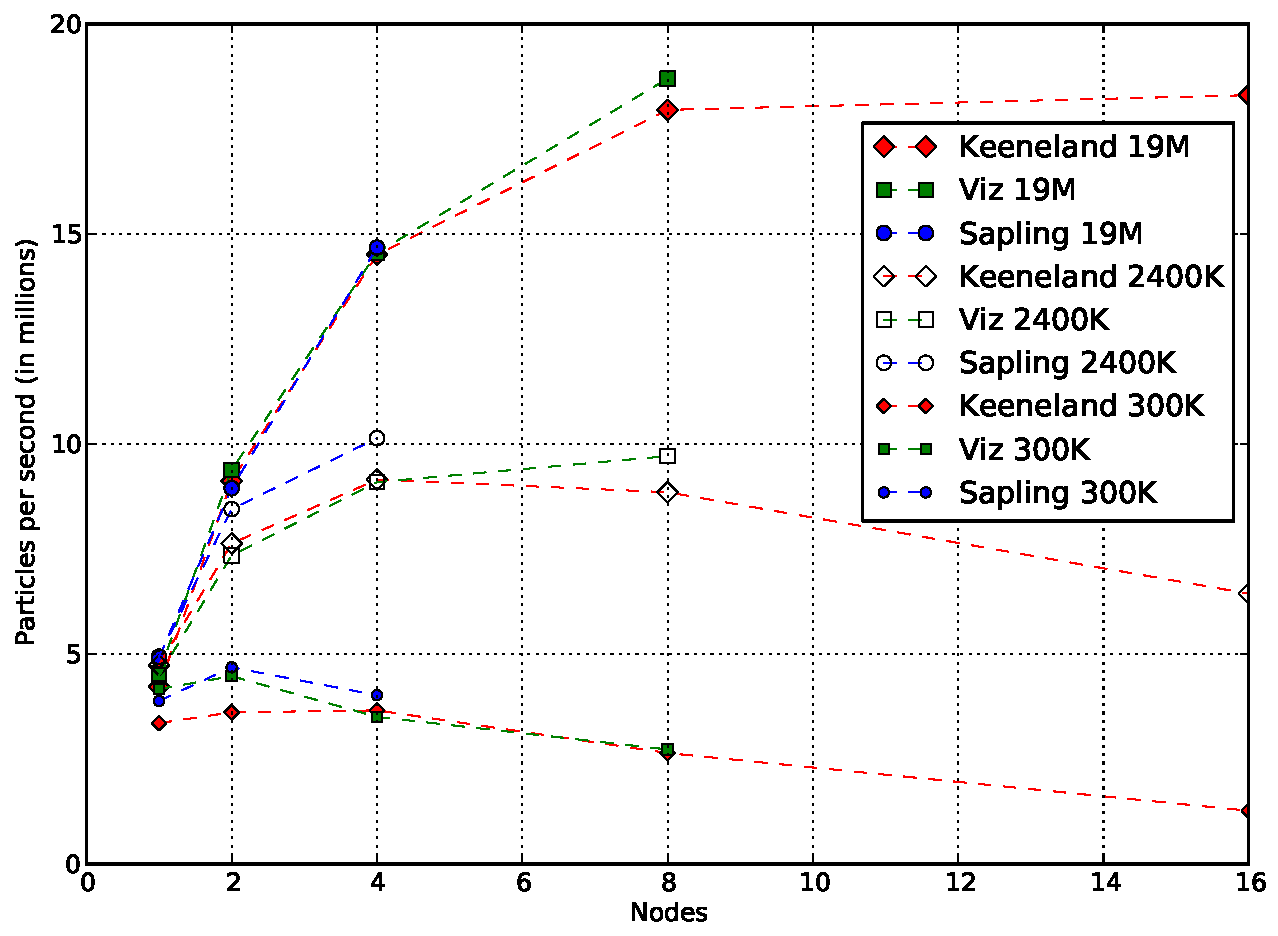
\includegraphics[scale=0.4]{figs/fluid_multinode.pdf}
\label{fig:fluid_multi}
}

%\subfigure[Effect of Load-Balanced Partitioning]
%{
%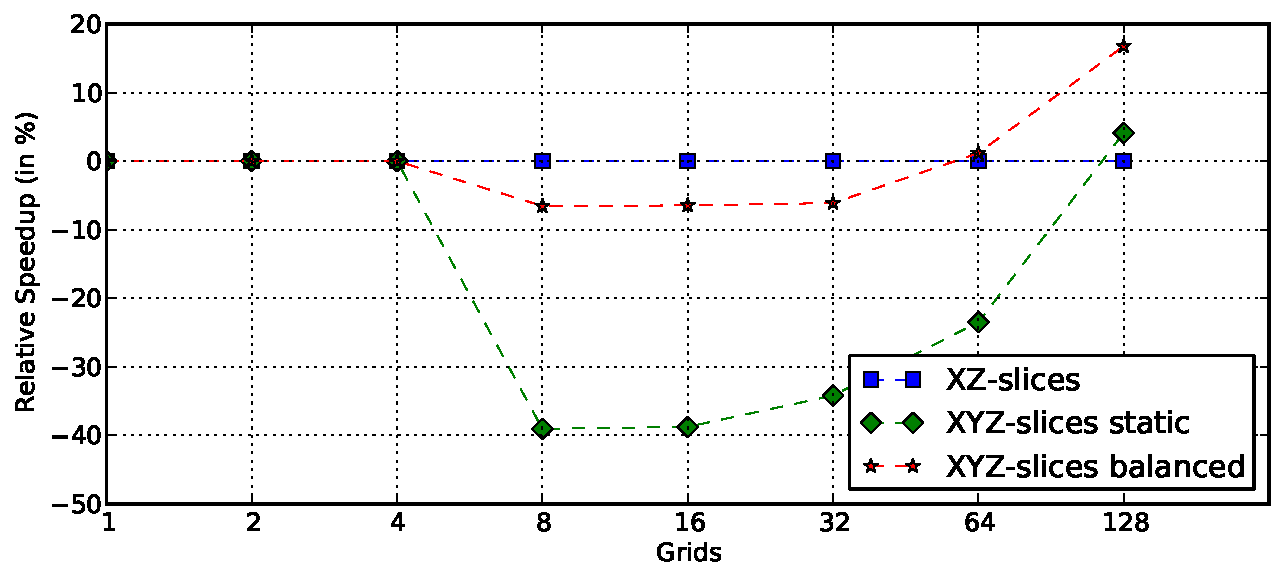
\includegraphics[scale=0.4]{figs/fluid_balance.pdf}
%\label{fig:fluid_balance}
%}
\caption{Fluid Simulation Results}
\end{figure}

\subsection{Adaptive Mesh Refinement}
\label{subsec:exp_amr}
Our final application is based on the third heat equation example from the Berkeley Labs 
BoxLib project \cite{BoxLib}.  This application is a three-level adaptive-mesh-refinement (AMR)
code that computes a first order stencil on a 2D mesh of cells.  The simulation iterates for many time
steps.  Updating the simulation for one time step consists of three phases.  In the first phase,
the boundary cells around a box at a refined level linearly interpolate their values from the nearby cells at the
next coarsest level.  The second phase computes the stencil computation on each cell in all levels.
In the third phase, cells at a coarser level that have been refined are restricted to the average
of the cells that they physically contain at the next finest level of refinement.

Achieving high-performance on this application is particularly challenging for several reasons.  
First, the application has a very high communication-to-computation ratio which, for a fixed problem
size begins as being memory bound and with increasing node count becomes network bound as the
perimeter-to-area ratio of cell grids increases.  Second, when choosing how to partition cells into grids, the
programmer must consider the locality both between cells in the same level, as well as for cells
across levels.  In the case of cross-level cell dependences, mapping decisions must be made at runtime as the
location of refinements are determined based on application input.  Finally, this application has
parallelism both between tasks running at the same level and tasks running across levels, leading
to complicated input-dependent data dependences.

BoxLib's implementation of this benchmark partitions cells within the same level into a number of grids
based on the number of nodes in the machine and distributes one grid from each level to each node.  This
optimizes for memory bandwidth and load balance, but does not take into account cross-level locality 
that exists between grids from different levels of refinement.  Furthermore, BoxLib does not block grids
into sub-grids to take advantage of intra-grid locality.

Our Legion implementation performs two optimizations that allow us to achieve better performance than BoxLib.
First, for each level of refinement we recursively partition the logical region of cells based on 
the number of nodes in the machine and the size of the L3 cache and L2 caches.  Legion allows us to describe 
locality for many levels of the memory hierarchy instead of just at the node-level.

Our second optimization takes advantage of the cross-level locality present in the application.  We implemented
an application specific mapper that inspects the arguments of tasks to discover the relationships between
grids at different levels of refinement.  The mapper dynamically performs intersection tests between logical regions
containing grids of different refinement levels to determine whether they overlap.  
If grids from different levels overlap, the mapper
ensures that they are always placed on the same node in the machine to leverage cross-level locality.  The mapper
memoizes the results of these intersection tests to amortize their cost.  The mapper also dynamically
load balances by distributing unconstrained grids from the coarsest level onto under-loaded nodes.

We compared our Legion implementation against BoxLib on three different problem sizes with a fixed number
of cells per level of refinement, but with randomly chosen refinements locations.  BoxLib also supports OpenMP
and we took their best number from using 1, 2, 4, or 8 OpenMP threads per node.  Our Legion implementation
always uses one thread per node to illustrate that in this application locality is significantly more important 
than parallelism.  The results from our experiments on all three clusters can be seen in Figure~\ref{fig:amr_total}. 

On just one node, blocking for caches using Legion achieves up to 2.6X speedup over BoxLib.  As the node count 
increases, the ability of our mapper to leverage cross-level locality allows us to further increase
our performance advantage to 5.4X over BoxLib by reducing the total communication costs.  

As the node count increased the AMR code becomes highly dependent on interconnect performance.  BoxLib performs much better
on Keeneland than it does on our viz cluster due to the better interconnect.  This can also be seen as we scale
to a larger number of nodes and BoxLib begins to catch up as can be seen in Figure~\ref{fig:amr_keeneland}.  
This occurs because our intra-level ghost-cell exchange algorithm relies on GASNet memory to exchange ghost cells which 
involves a linear increase in network traffic with the number of nodes.  BoxLib instead uses direct
node-to-node exchanges of ghost cells similar to our fluid application.  A future implementation of our AMR code 
will employ a similar ghost cell exchange algorithm to improve scalability.

\begin{figure}
\subfigure[Sapling Results]
{
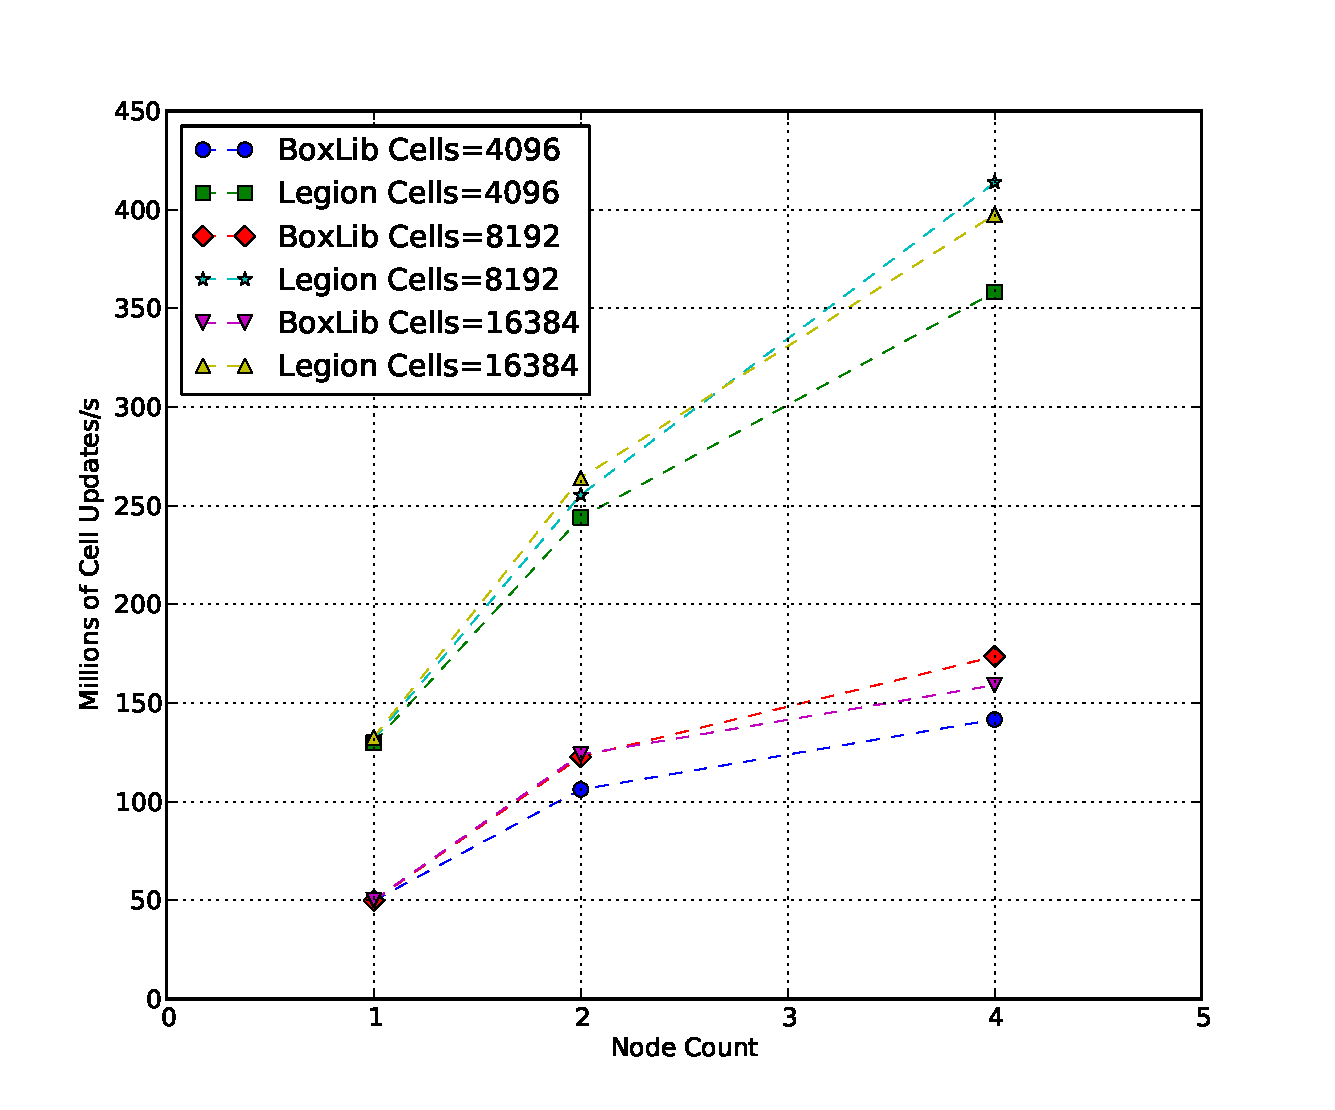
\includegraphics[scale=0.4]{figs/Sapling_amr.pdf}
\label{fig:amr_sapling}
}

\subfigure[Viz Results]
{
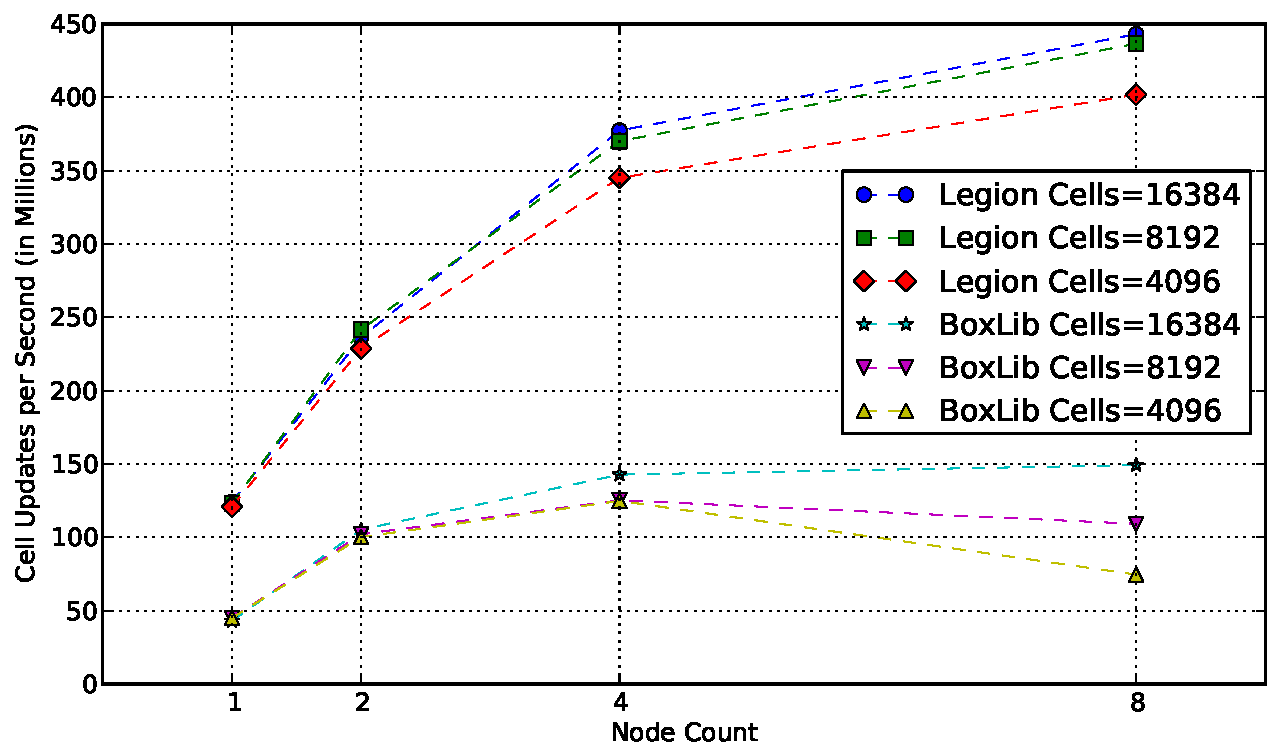
\includegraphics[scale=0.4]{figs/Viz_amr.pdf}
\label{fig:amr_viz}
}

\subfigure[Keeneland Results]
{
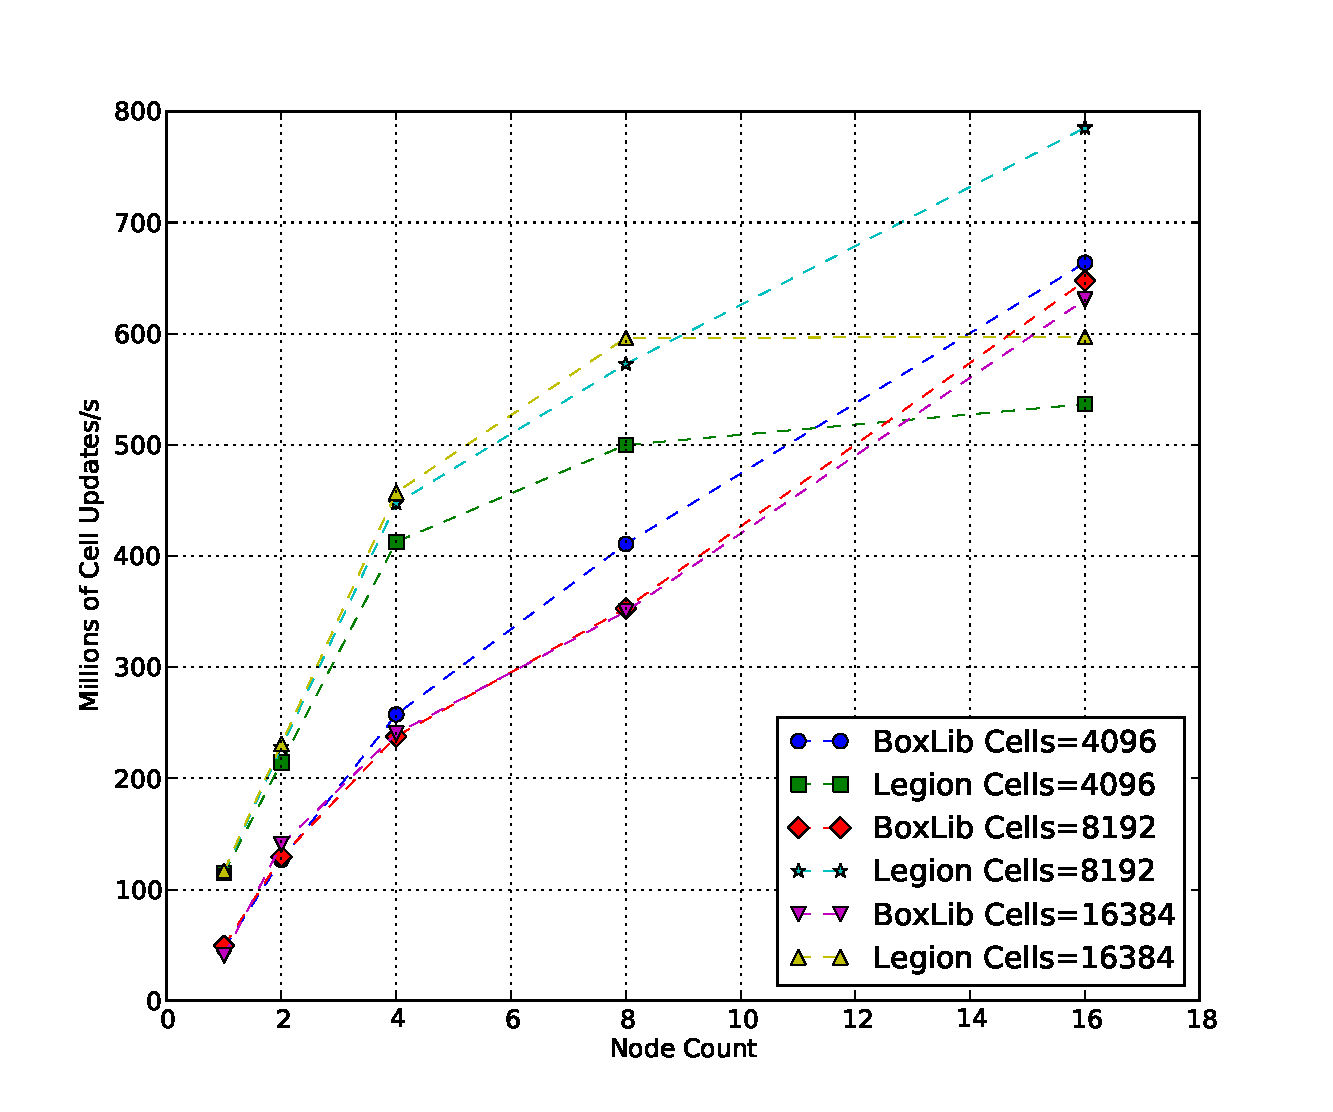
\includegraphics[scale=0.4]{figs/Keeneland_amr.pdf}
\label{fig:amr_keeneland}
}
\caption{Throuphput of Adaptive Mesh Refinement in Millions of Cells/s \label{fig:amr_total}}
\end{figure}
